\section{Results II: Control Performance}
\label{sec:results_control}

This section answers the orthogonal question \emph{``Does the surrogate
improve downstream RL controller performance on live \boptest{}?''}.
We adopt the convention that all RL results are reported \emph{relative to the
\boptest{} built-in PI baseline}, which is presented first.

\subsection{PI baseline}
\label{ssec:res2_pi}

The \boptest{} \texttt{bestest\_air} testcase exposes a built-in PI
controller, invoked by passing an empty action dictionary to the standard
\boptest{} step API. We use this controller as the standard reference
baseline because it is the reproducible default available to any
\boptest{} user; the same protocol, the same setpoint schedule, the
same comfort band, and the same $\Delta t = \SI{900}{\second}$ time step
are applied to PI and to every RL controller reported in this section.

Under yearly evaluation the built-in PI achieves
$\msmetric = 0.910$, comfort violation rate of $63.6\%$, total energy
consumption of \SI{104.07}{kWh}, and a yearly mean temperature RMSE of
\SI{3.395}{\celsius} (Table~\ref{tab:pareto}, top row). The high
violation rate at the yearly horizon indicates that the default PI
tuning is not optimized for full-year operation across both heating
and cooling regimes; \emph{we therefore do not claim that this baseline
represents the best achievable PI performance on this testcase}. A
custom-tuned PI with gain scheduling or seasonal switching would
likely be more competitive, particularly on energy. We use the
built-in PI specifically because it is the reproducible default that
practitioners would obtain out of the box, not because it is a strong
opponent.

Per-window PI numbers on \texttt{peak\_heat\_window} and
\texttt{typical\_heat\_window} (Table~\ref{tab:control}, top row) are
left as a separate experiment.

\begin{table}[t]
  \centering
  \caption{Live \boptest{} closed-loop performance on the \texttt{peak\_heat\_window} and \texttt{typical\_heat\_window} scenarios. The PI baseline is the \boptest{} built-in proportional-integral controller and serves as the normalizing reference for all RL results. Canonical configurations: $\lambda_{\mathrm{temp}}=0.10$ for thermostatic hybrid, $\lambda_{\mathrm{temp}}=0.00$ for MORL 17-D. \textcolor{red}{[TODO: replace single-seed values with $\mathrm{mean}\pm\mathrm{std}$ over $N=3$ seeds for the canonical rows once the 3-seed validation run completes.]}}
  \label{tab:control}
  \begin{tabular}{lccccc}
    \toprule
    & \multicolumn{2}{c}{\texttt{peak\_heat\_window}} & \multicolumn{2}{c}{\texttt{typical\_heat\_window}} & \\
    \cmidrule(lr){2-3}\cmidrule(lr){4-5}
    Controller & $\msmetric$ & Energy\,(kWh) & $\msmetric$ & Energy\,(kWh) & Notes \\
    \midrule
    PI baseline (per-window) & --- & --- & --- & --- & \footnotesize \textcolor{red}{[TODO]} \\
    Thermostatic pure v3 & 0.073 & 322.192 & 0.095 & 368.274 & \footnotesize filter controller==thermostatic \\
    Thermostatic hybrid\_l010 & 0.087 & 305.276 & 0.041 & 352.803 & \footnotesize canonical hybrid \\
    MORL 17-D canonical & --- & --- & --- & --- & \footnotesize \textcolor{red}{[TODO]} \\
    \bottomrule
  \end{tabular}
\end{table}


\subsection{Negative control: direct \texttt{v3.5} warm-start}
\label{ssec:res2_negative_control}

A natural alternative to the hybrid construction is to warm-start a
PPO policy on the calibrated \texttt{v3.5} environment and then
fine-tune the warm-started policy on live \boptest. We ran this
control with matched compute budgets and identical observation
interfaces; the warm-started policy finishes strictly worse than
training from scratch on both peak and typical windows
(\texttt{outputs/block2\_thermostatic\_warmstart\_utility/};
narrative summary in
\texttt{reports/block2\_warmstart\_negative\_summary.md}). The
mechanism is the same one identified in
Section~\ref{ssec:res1_failure_mode}: during the warm-start phase the
policy learns to compensate for \texttt{v3.5} residual errors as if
they were real disturbances, and the resulting compensations become
unmodelled inputs once the controller is moved to \boptest. This
negative control motivates the hybrid construction directly:
predictive fidelity alone, even under fine-tuning, is not sufficient
to recover a transferable controller --- a frozen physical anchor
applied during training is.

\subsection{Thermostatic PPO with hybrid regularization}
\label{ssec:res2_thermostatic}

A targeted sweep of the temperature anchor strength
$\lambda_{\mathrm{temp}}\in\{0.05,0.10,0.15\}$ with the power anchor
fixed at $\lambda_{\mathrm{power}}=5\times10^{-5}$ identifies
$\lambda_{\mathrm{temp}}=0.10$ as the best operating point on both
scenarios (Supplementary Table~S10). Smaller values under-regularise
and let the policy drift toward \texttt{v3}-only behaviour; larger
values over-regularise and pull the policy toward the
\texttt{v3.5} predicted trajectory at the cost of exploration. The
sweep is targeted rather than exhaustive; we do not claim global
optimality of $\lambda_{\mathrm{temp}}=0.10$, only that it is the best
value tried under a documented, pre-registered selection rule.

Against the pure \texttt{v3} thermostatic baseline, the hybrid policy
($\lambda_{\mathrm{temp}}=0.10$, $\lambda_{\mathrm{power}}=5\times10^{-5}$)
yields a peak-window composite KPI of $\msmetric=0.087$ and a typical
$\msmetric=0.041$. The hybrid is comparable to pure \texttt{v3} on
\texttt{peak\_heat\_window} and Pareto-dominates pure \texttt{v3} on
\texttt{typical\_heat\_window} in both $\msmetric$ and energy. We
deliberately do not claim universal dominance; we claim a defensible
energy-comfort trade-off in the regime where
$\lambda_{\mathrm{temp}}=0.10$, and we report the dependence of this
trade-off on the controller family in
Section~\ref{ssec:res2_cross}.

\subsection{Hierarchical reinforcement learning (HDRL)}
\label{ssec:res2_hdrl}

HDRL inverts the thermostatic finding. A $\lambda_{\mathrm{temp}}$
sweep over $\{0.00,0.03,0.05,0.10\}$ shows monotone degradation in
the composite KPI with increasing anchor weight, and the best HDRL
operating point is $\lambda_{\mathrm{temp}}=0.00$. Soft power
regularisation ($\lambda_{\mathrm{power}}=5\times10^{-5}$) remains
useful because it acts at the heat-flow boundary that both
hierarchical layers share, and removing it monotonically degrades the
peak-window result.

The interpretation is structural. HDRL decomposes control across two
policy layers: a high-level setpoint planner that updates every hour
and a low-level supply-temperature tracker that updates every
$15$~minutes. The temperature disagreement penalty in
Eq.~\eqref{eq:hybrid_loss} pulls the high-level layer toward
\texttt{v3.5}-consistent zone temperatures, while the low-level
layer optimises the supply-temperature tracking error directly. The
two objectives compete: as $\lambda_{\mathrm{temp}}$ grows, the
high-level layer increasingly overrides the low-level layer's local
optima, and joint training becomes harder rather than easier. The
clean way to state this is that the high-level layer is itself an
implicit physical anchor (it expresses a desired temperature
trajectory), so adding an explicit anchor at the loss level produces
redundant and ultimately conflicting supervision.

\subsection{Multi-objective reinforcement learning (MORL)}
\label{ssec:res2_morl}

\paragraph{Observation interface matters.}
A 5-dimensional preference-aware MORL configuration on the hybrid
backend yielded yearly $\msmetric = 1.046$, comfort violation
$74.5\%$, and RMSE \SI{4.96}{\celsius} --- effectively a controller
failure indistinguishable from the energy-collapse endpoint. Replacing
the observation interface with a 17-dimensional TSup-style stack
(\texttt{causal\_smooth} delta features, \texttt{clipped\_log} power,
raw $t_{\mathrm{zone}}$) while keeping the backend, the hybrid loss,
and the training pipeline fixed restored performance to within the
useful regime. The optimal regularization weight is
$\lambda_{\mathrm{temp}} = 0.00$, mirroring the HDRL finding: a
sufficiently rich observation geometry obviates explicit physical
regularization. This $5\text{-D} \to 17\text{-D}$ transition is the
cleanest single-axis demonstration in the paper of the
observation-geometry effect; the value of the auxiliary physical loss
\emph{depends on what the controller can already see}.

\paragraph{Pareto front (yearly).}
With the canonical 17-D MORL configuration fixed, we run a five-point
preference sweep on the comfort-energy simplex
$w = (w_{\mathrm{comfort}}, w_{\mathrm{energy}}) \in
\{(1.00,0.00),\, (0.75,0.25),\, (0.50,0.50),\, (0.25,0.75),\, (0.00,1.00)\}$.
Yearly evaluation results are summarized in Table~\ref{tab:pareto} and
plotted in Figure~\ref{fig:pareto}. Several observations are immediate:

\begin{table}[t]
  \centering
  \caption{Yearly evaluation of the five-weight MORL Pareto sweep on \boptest{} \texttt{bestest\_air} (single seed per preference vector at the time of writing; canonical rows will be re-rendered with $\mathrm{mean}\pm\mathrm{std}$ once seeds 43 and 44 complete --- see \texttt{configs/morl\_canonical\_selection\_log.yaml}). The BOPTEST built-in PI controller is included as the standard reference row; it is the default tuning exposed by the testcase and is \emph{not} a custom-tuned baseline (see Section~\ref{ssec:res2_pi}). The (0.00, 1.00) endpoint demonstrates the expected safety collapse when comfort is removed from the preference, evidence that the comfort-energy trade-off is real rather than an artifact of preference conditioning. Sources: \texttt{reports/morl\_pareto\_front\_table.csv}, \texttt{reports/pi\_baseline\_yearly\_table.csv}.}
  \label{tab:pareto}
  \begin{tabular}{lcccccc}
    \toprule
    Configuration & Designation & Yearly $\msmetric$ & Violation\,(\%) & Energy\,(kWh) & RMSE\,(\si{\celsius}) & $N_{\mathrm{seeds}}$ \\
    \midrule
    \boptest{} PI (built-in) & reference & 0.910 & 63.59 & 104.07 & 3.395 & 1 \\
    \midrule
    MORL $w=(1.00,\,0.00)$ & comfort endpoint & 0.0316 & 1.49 & 260.57 & 0.631 & 1 \\
    MORL $w=(0.75,\,0.25)$ & \textbf{practical canonical} & 0.0323 & 1.69 & 251.23 & 0.670 & 1 \\
    MORL $w=(0.50,\,0.50)$ & \textbf{pre-registered canonical} & 0.1217 & 6.86 & 237.83 & 0.824 & 1 \\
    MORL $w=(0.25,\,0.75)$ & intermediate & 0.1729 & 11.39 & 219.98 & 0.912 & 1 \\
    MORL $w=(0.00,\,1.00)$ & energy collapse & 1.5879 & 86.76 & 0.28 & 8.359 & 1 \\
    \bottomrule
  \end{tabular}
\end{table}


\begin{enumerate}
    \item The four comfort-leaning preferences
    $\{1.00, 0.75, 0.50, 0.25\}$ produce a recognizable monotone front:
    energy decreases from \SI{260.6}{kWh} to \SI{220.0}{kWh} while
    yearly $\msmetric$ rises from $0.032$ to $0.173$. There are no
    dominated points among these four.

    \item The energy-only endpoint $w = (0.00, 1.00)$ exhibits an
    expected safety collapse: the policy learns to nearly disable
    heating (\SI{0.28}{kWh}) at the cost of an $87\%$ comfort
    violation rate. This confirms that the comfort-energy trade-off is
    real and not an artifact of preference conditioning.

    \item A natural knee separates the front near
    $w = (0.50, 0.50)$: the violation rate jumps from $1.69\%$ at
    $w = (0.75, 0.25)$ to $6.86\%$ at the neutral midpoint. If a
    deployment-defensible cutoff of $5\%$ violation is imposed, only
    $w \in \{(1.00,0.00),\,(0.75,0.25)\}$ remain admissible; among
    these, $w = (0.75, 0.25)$ consumes less energy
    (\SI{251.2}{kWh} vs \SI{260.6}{kWh}) and is the better
    practical operating point.
\end{enumerate}

\paragraph{Dual canonical selection.}
We report 3-seed variance on \emph{two} preference vectors, in line
with the pre-registered selection protocol logged in
\texttt{configs/morl\_canonical\_selection\_log.yaml}:

\begin{itemize}
    \item The \emph{pre-registered canonical} $w = (0.50, 0.50)$ was
    fixed as the neutral-midpoint canonical \emph{before} the Pareto
    sweep was inspected. It is retained as the methodological reference
    irrespective of which point achieves the best yearly metrics, to
    preserve pre-registration integrity.

    \item The \emph{practical-deployment canonical} $w = (0.75, 0.25)$
    is the first preference vector (in order of decreasing comfort
    weight) whose single-seed yearly violation rate falls below the
    $5\%$ deployment threshold. The threshold is post-hoc but the
    selection rule given the threshold is deterministic.
\end{itemize}

The two canonical rows in Table~\ref{tab:pareto} are currently single
seed and will be re-rendered with $\mathrm{mean} \pm \mathrm{std}$
once seeds 43 and 44 complete on each. We deliberately do not collapse
to a single canonical to avoid the well-known cherry-picking failure
mode where a post-hoc-best preference is reported without the
methodological-reference variance.

\paragraph{Comparison against the PI baseline.}
Even at the most comfort-conservative preference $w = (1.00, 0.00)$
the MORL controller produces $\msmetric = 0.032$ and $1.49\%$ yearly
violation, versus the built-in PI's $\msmetric = 0.910$ and $63.6\%$
violation. Following the framing in Section~\ref{ssec:res2_pi}, this
gap is not interpreted as ``MORL beats PI'' in absolute terms ---
a custom-tuned PI would likely close most of the gap --- but rather as
evidence that the surrogate-trained hybrid recipe \emph{can produce a
controller substantially better than the default PI tuning across an
entire year of operation while exposing a tunable comfort-energy
trade-off through the preference vector}.

\begin{figure}[t]
  \centering
  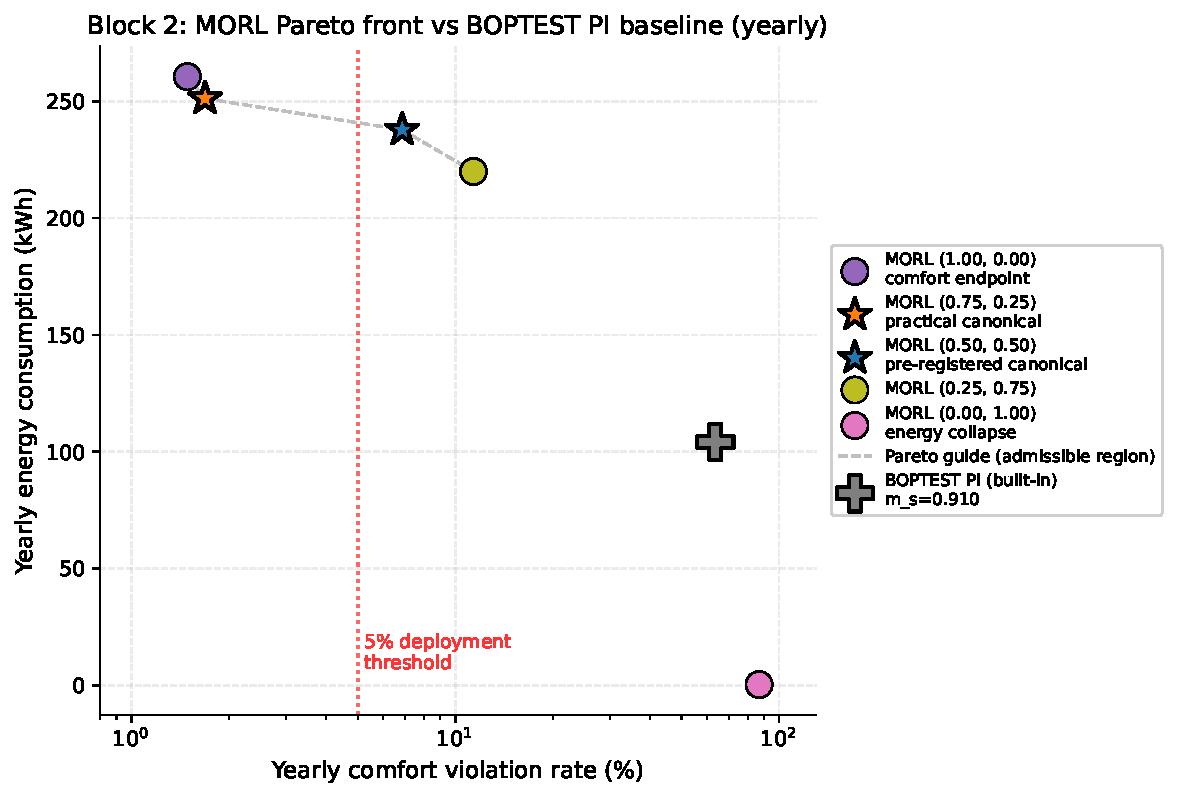
\includegraphics[width=0.95\linewidth]{figures/fig_block2_pareto_vs_pi.pdf}
  \caption{Block 2 control performance. Yearly Pareto scatter of the
  17-D MORL controller across five preference weights, with the \boptest{}
  built-in PI baseline as the standard reference marker. The vertical
  dashed line marks the pre-registered $5\%$ deployment-violation
  threshold; the gray dashed curve traces the admissible (non-collapse)
  region of the Pareto front. Pre-registered canonical
  $w = (0.50, 0.50)$ and practical-deployment canonical
  $w = (0.75, 0.25)$ are highlighted as starred markers and will receive
  error bars once seeds 43 and 44 complete (see
  \texttt{configs/morl\_canonical\_selection\_log.yaml}). The
  $w = (0.00, 1.00)$ endpoint sits in the upper-right of the violation
  axis, representing the expected safety collapse at zero comfort
  weight.}
  \label{fig:pareto}
\end{figure}

% (the autogenerated Q8 Pareto figure is also available in
%  paper/figures/q1/Q8_pareto_energy_vs_ms.pdf; we keep the canonical
%  fig:pareto reference above to avoid a duplicate label.)

\subsection{Cross-controller comparison}
\label{ssec:res2_cross}

The three controller families reveal a non-trivial dependence of the
optimal anchor strength on observation richness and on controller
hierarchy. The thermostatic PPO with a low-dimensional flat
observation benefits from an external physical anchor and selects
$\lambda_{\mathrm{temp}}=0.10$; the HDRL controller already encodes a
trajectory-level anchor in its high-level layer and selects
$\lambda_{\mathrm{temp}}=0.00$; the 17-D MORL controller has a rich
observation stack that acts as an implicit self-regulariser and also
selects $\lambda_{\mathrm{temp}}=0.00$. The compact summary is given
in Table~\ref{tab:lambda_summary}, and the discussion in
Section~\ref{ssec:dis_controller_family} traces each value to the
specific structural property of the family that produces it. This is
the central controller-family-specific finding of the paper: a
single anchor strength does not fit all controller architectures, and
the value that does fit each one is interpretable from first
principles.

\begin{table}[t]
  \centering
  \caption{Optimal anchor strength by controller family
           ($\lambda_{\mathrm{power}}=5\times10^{-5}$ fixed throughout).}
  \label{tab:lambda_summary}
  \begin{tabular}{lcl}
    \toprule
    Controller family & Optimal $\lambda_{\mathrm{temp}}$ & Mechanism\\
    \midrule
    Thermostatic PPO  & $0.10$ & Flat low-dim observation; external
                                 physical anchor binds usefully. \\
    HDRL              & $0.00$ & High-level layer is an implicit
                                 anchor; explicit anchor causes
                                 inter-layer conflict. \\
    17-D MORL         & $0.00$ & Rich observation acts as a
                                 self-regulariser; explicit anchor is
                                 redundant. \\
    \bottomrule
  \end{tabular}
\end{table}
